\section{Modelado del Sistema}\label{sec:modelo}

En la figura \ref{fig:statemachine}, se muestra el modelo del sistema que se va a
desarrollar como una m\'aquina de estados con cinco componentes
diferencidos:

\begin{itemize}
\item Las componentes BH1750 y DTH22 est\'an compuestas por dos
  estados: En \emph{S0} el sensor est\'a midiendo la magnitud f\'isica
  correspondiente y en \emph{S1} el sensor env\'ia los datos medidos
  al Arduino Uno al que est\'a conectado, volvi\'endose al estado
  \emph{S0} para comenzar una nueva medici\'on.
\item Los Arduinos Uno est\'an compuestos por tres estados: En
  \emph{S2} se reciben los datos del sensor, en \emph{S3} se procesan
  para mandarlos de manera unificada usando la estructura de datos
  Data (definida en Comm.h) y, finalmente, en \emph{S4} se env\'ian
  los datos a la Discovery, volviendo a esperar nuevos datos en
  \emph{S2}.
\item La Discovery SMT32 est\'a formada por tres estados: \emph{S5}
  espera a recibir datos de uno de los Arduinos. Una vez que los
  recibe, los procesa en el estado \emph{S6} y, finalmente, se produce
  la visualizaci\'on de los mismos en \emph{S7}. 
\end{itemize}

\begin{center}
\begin{figure}[h]\label{fig:statemachine}
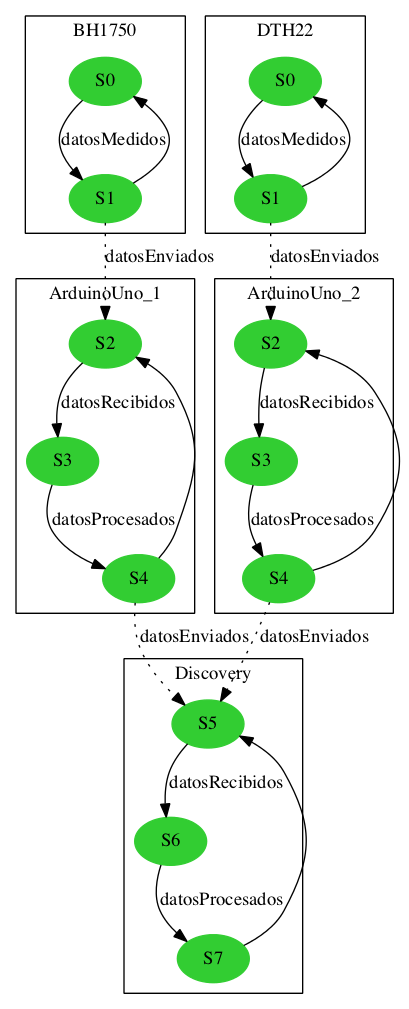
\includegraphics{images/maquina_estados.png}
\caption{M\'aquina de estados}
\end{figure}
\end{center}
